\documentclass[../main.tex]{subfiles}
\addbibresource{../bibfile.bib}

\begin{document}


\chapter{Stato dell'arte}
\markboth{Capitolo 2}{}
\label{chap:related}
Questo capitolo tratta una rassegna di alcune metodologie, tecniche e soluzioni attualmente disponibili per risolvere il problema della ricerca automatica di vulnerabilità in file binari.
Verranno in particolare approfonditi alcuni approcci basati su analisi statica, analisi dinamica e su tecniche di apprendimento automatico.
Per ciascuna metodologia presentata, verranno dettagliati il suo funzionamento generale, le sue capacità di analisi e le sue limitazioni

\section{Metodologie basate su tecniche di analisi statica}
L'analisi statica di un programma consiste in un insieme di metodologie, tool e algoritmi che permettono l'analisi del codice sorgente o della
sua rappresentazione binaria (per esempio, un file eseguibile) senza che il programma venga effettivamente eseguito \cite{static_analysis_introduction}.
Questa tecnica è ampiamente adottata nell'ambito della ricerca delle vulnerabilità, in quanto consente di inferire e determinare se
certe proprietà sono soddisfatte (per esempio, le condizioni che possono portare ad una certa vulnerabilità) senza direttamente eseguire il programma.
Tuttavia, l'analisi statica condotta direttamente su un file binario è intrinsecamente più complessa rispetto all'analisi statica del codice sorgente:
le principali difficoltà risiedono nella mancanza di informazioni riguardante i tipi e la struttura ad alto livello del codice \cite{Review_of_static_analysis} e nella necessità di gestire e rappresentare adeguatamente le operazioni riguardanti la memoria \cite{CodeSurfer}.
Nonostante queste sfide, nel corso degli anni sono stati sviluppati diversi approcci e metodologie di analisi statica progettati per effettuare la ricerca di vulnerabilità all'interno di file binari.
Queste tecniche, tuttavia, possono produrre un elevato numero di falsi positivi e falsi negativi : poiché non effettuano un'esecuzione concreta del programma,
esse devono effettuare diverse assunzioni sul suo stato a runtime. Ciò potrebbe quindi portare i tool basati su questa tipologia di analisi a segnalare vulnerabilità in porzioni di programma non vulnerabili.
\subsection{Taint analysis statica}
La \textit{taint analysis} (o \textit{taint checking}) è una tecnica di analisi che mira a tracciare e monitorare la propagazione di flussi di dati inaffidabili o 
potenzialmente dannosi all'interno del programma. La taint analysis si compone di tre elementi chiave:
\begin{enumerate}
    \item \textbf{Sorgenti} (Sources): Sono i punti del programma dove si origina un flusso di dati inaffidabile. Una sorgente potrebbe per esempio essere l'input di un utente oppure i dati
    letti da un file.
    \item \textbf{Propagazione}: Viene effettuato un monitoraggio continuo della propagazione nel programma dei dati provenienti da una sorgente
    \item \textbf{Sink}: Sono i punti del programma che effettuano operazioni sensibili, come per esempio l'accesso al filesystem o la chiamata ad operazioni di libreria non sicure. 
\end{enumerate}
Una possibile vulnerabilità verrà quindi rilevata quando il programma permette ad un dato "tainted" di raggiungere un sink; ciò può avvenire quando, per esempio, il dato
non viene adeguatamente sanificato.
\newline
\textbf{Bintaint} è un tool di parsing capace di effettuare taint analysis statica su file binari  \cite{Bintaint}.
Il taint analyzer proposto è basato sul tool commerciale di reverse engineering \textit{IDA}, il quale viene utilizzato per recuperare il codice assembly dal codice binario, 
ed è implementato utilizzando il linguaggio funzionale \textit{OCaml}.
Bintaint è composto da quattro moduli distinti:
\begin{itemize}
    \item \textbf{Decoder module}: Questo modulo si occupa di tradurre il codice assembly recuperato da IDA in una rappresentazione in un linguaggio intermedio chiamato \textit{REIL} (Reverse Engineering Intermediate Language), 
    le quali espressioni verranno a loro volta convertite in espressioni simboliche.
    \item \textbf{Taint Processing Configuration Module}: Questo modulo gestisce la configurazione per l'inizializzazione della taint analysis, leggendo la configurazione fornita dall'utente in formato XML, la quale
    dovrà contenere tutte le informazioni necessarie per effettuare la taint analysis. Questo modulo si occupa inoltre di stabilire una relazione tra l'input esterno e le varie sorgenti definite
    \item \textbf{Expression Parsing Module}: Questo modulo si occupa di definire come avviene la propagazione dei flussi di dati tainted all'interno del programma
    \item \textbf{TCFG Generation Module}: Questo modulo si occupa di generare una struttura a grafo diretta chiamata \textit{Taint Control Flow Graph}, la quale rappresenterà tutte le possibili aree del programma che un determinato flusso tainted può raggiungere.
    L'analisi del TCFG permetterà quindi di evincere se un determinato sink dipende dai dati generati da una determinata sorgente.
\end{itemize}
L'approccio proposto dal tool permette di ridurre il numero di falsi positivi e falsi negativi rilevati rispetto ad una tain analysis tradizionale; inoltre, l'utilizzo del linguaggio intermedio REIL
permette al tool di essere facilmente integrabile in sistemi di analisi più complessi, a patto che anch'essi utilizzino lo stesso linguaggio di rappresentazione intermedia. 
Tuttavia il tool risulta comunque dipendente dall'input dell'analista; l'accuratezza dell'analisi dipenderà quindi dalla corretta definizione di sorgenti, sink e propagazione da parte
di quest'ultimo. Infine, Bintaint si basa sul framework commerciale IDA, il quale non offre tutte le sue funzionalità nella sua versione gratuita.
\subsection{Binary Code Similarity Detection}
Quando l'obbiettivo dell'analisi è ricercare una vulnerabilità nota (per esempio, una debolezza già documentata), è possibile adottare una strategia chiamata \textit{Binary Code Similarity Detection} (BCSD).
Questo approccio si basa sul confronto il codice binario del programma in esame con la firma (il codice binario) della vulnerabilità.
Se l'algoritmo di analisi rileva segmenti di codice con un elevato grado di somiglianza con la firma della vulnerabilità, allora è altamente probabile che il programma
contenga quella vulnerabilità. Un algoritmo di decisione determinerà se il programma contiene effettivamente la vulnerabilità.
Tuttavia, poiché il codice contente la vulnerabilità spesso richiede solo piccole modifiche per fare in modo che esso non sia più vulnerabile (l'aggiunta di un controllo, l'impostazione di permessi aggiuntivi, ...), il codice binario del programma corretto e il programma originale
saranno molto simili; potenzialmente portando l'analizzatore a segnalare dei falsi positivi \cite{Survey_of_Binary_Code_Security_Analysis}. \newline
\textit{VulneraBin} \cite{VulneraBin} è un tool che effettua un'analisi BCSD attraverso una metrica di similarità basata su hashing, strutturando il processo nelle seguenti fasi:
\begin{enumerate}
    \item \textbf{Re-ottimizzazione del linguaggio di rappresentazione intermedia (IR)}: Il codice assembly viene dapprima tradotto nel linguaggio di rappresentazione intermedia VEX-IR, il quale utilizzo
    mira ad appiattire le eventuali differenze sintattiche derivanti dall'utilizzo di registri diversi, istruzioni diverse per l'assegnamento o metodologie di ottimizzazione introdotte dai vari compilatori.
    Successivamente, viene applicata un'ulteriore ottimizzazione sul codice intermedio per eliminare le differenze residue che potrebbero ancora persistere a causa delle diverse tecniche di ottimizzazione dei compilatori.
    \item \textbf{Program Slicing}: Il program slicing è una tecnica di anali statica che, partendo da un sottoinsieme dei comportamenti di un programma, ne produce una versione minimale, chiamata "slice",  la quale mantiene esattamente lo stesso sottoinsieme di comportamenti.
    Poiché questa tecnica è alla base delle analisi offerte dalla piattaforma, verrà ulteriormente approfondita nel \textit{Capitolo 3} di questa tesi.
    \item \textbf{Strand normalization}: Una "strand" è definita come l'insieme di istruzioni contigue richieste per computare il valore di una specifica variabile \cite{Statistical_similarities_in_binaries}.
    Gli strand vengono normalizzati rinominando i registri utilizzati durante le varie operazioni, andando così ad eliminare eventuali differenze sintattiche introdotte dai compilatori
    \item \textbf{Similarity evaluation}: Viene effettuato un confronto fra gli hash MD5 calcolati sugli strand normalizzati e gli hash delle vulnerabilità contenute in un database. Se la similarità supera una certa soglia definita manualmente, allora
    il binario sarà considerato vulnerabile.
\end{enumerate}
\begin{figure}[h]
    \centering % Questo comando centra il contenuto orizzontalmente
    \scalebox{0.8}{ % Scaling a 80% per adattarsi alla larghezza della pagina
        \begin{tikzpicture}[
            % Stili dei nodi
            % Riduzione della larghezza minima e della text width
            block/.style={rectangle, draw, minimum height=1.2em, minimum width=5em, align=center, text width=5em, font=\small},
            output/.style={font=\small}, 
            % Stili delle frecce
            line/.style={draw, -{Stealth}, thick}
        ]

            % 1. Nodi del diagramma
            \node (query) [output] {Query};
            % Riduzione della spaziatura tra i blocchi a 1cm
            \node (lift) [block, right=0.5cm of query] {Lift \& re-optimize};
            \node (slicing) [block, right=0.5cm of lift] {Slicing};
            \node (normalize) [block, right=0.5cm of slicing] {Normalize};
            % text width leggermente ridotta
            \node (hash) [block, right=0.5cm of normalize, text width=6em] {Calculate hash value \& evaluate weight};
            \node (search) [block, right=0.5cm of hash] {Search in database};
            \node (output) [output, right=0.5cm of search] {Output};

            % 2. Connessioni (frecce)
            \path[line] (query) -- (lift);
            \path[line] (lift) -- (slicing);
            \path[line] (slicing) -- (normalize);
            \path[line] (normalize) -- (hash);
            \path[line] (hash) -- (search);
            \path[line] (search) -- (output);

        \end{tikzpicture}
    }
    \caption{Schema di funzionamento di VulneraBin. Immagine proveniente da \cite{VulneraBin}}
\end{figure}
Nonostante l'approccio proposto porti ad un miglioramento della complessità computazionale dell'analisi e alla mitigazione del numero di falsi positivi e negativi rilevati, l'affidabilità dell'analisi rimane comunque legata ad una soglia scelta manualmente dall'analista.
Sarà quindi necessario che quest'ultimo imposti una soglia ottimale per ogni specifico binario o classe di vulnerabilità, compromettendo quindi l'automazione del processo.
\section{Metodologie basate su tecniche di analisi dinamica}
L'analisi dinamica consiste nell'osservazione del comportamento di un programma mentre esso viene eseguito in un determinato ambiente d'esecuzione.
Per consentire questo tipo di analisi, i tool che implementano questo tipo di tecniche devono effettuare un processo chiamato \textit{instrumentation}, il quale
consiste nell'aggiungere codice di analisi all'interno del programma da analizzare in modo tale che venga eseguito insieme a quest'ultimo senza modificarne il normale
flusso di esecuzione \cite{DBA_DBI}. I risultati ottenuti tramite l'analisi dinamica sono generalmente più precisi rispetto ai risultati ottenuti effettuando un'analisi statica
del programma, poiché non vi è più la necessità di effettuare un'astrazione riguardo i valori computati o il cammino intrapreso dal programma sotto analisi.
Tuttavia, poiché l'esecuzione concreta di un programma richiede la scelta di un insieme di input concreti con il quale eseguirlo, i risultati ottenuti tramite queste tecniche non sono
generalizzabili, in quanto l'insieme di input scelto potrebbe non essere rappresentativo di tutti i possibili cammini d'esecuzione del programma \cite{Synergy_Duality}.
\subsection{Fuzzing}
Il fuzzing è una tecnica di analisi dinamica che consiste nell'osservare il comportamento del programma quando esso
riceve degli input casuali o malformati. Se un input provoca un blocco dell'esecuzione o un crash, allora il programma
potrebbe allora contenere una problematica di implementazione oppure una debolezza software, la quale, sotto certe circostanze, potrebbe
risultare sfruttabile da un potenziale attaccante.
Questa tecnica viene implementata attraverso programmi specializzati, chiamati \textit{fuzzers}; un esempio noto è \textbf{American Fuzzy Lop} (AFL).
Generalmente, i principali componenti del fuzzing (e di un fuzzer) sono\cite{Fuzzing_soa}:
\begin{itemize}
    \item \textbf{Programma obbiettivo}: Il programma da analizzare, il quale può essere rappresentato sia dal suo codice binario sia dal suo codice sorgente. Poiché l'accesso a quest'ultimo è a volte ostico in situazioni reali, i software di fuzzing hanno spesso
    come programma obbiettivo il solo codice binario.
    \item \textbf{Monitor}: Raccoglie informazioni riguardanti l'esecuzione del programma.
    \item \textbf{Input generator}: Si occupa della generazione degli input, la quale può avvenire in due modi distinti:
    \begin{itemize}
        \item \textbf{Grammar-based}: Gli input vengono generati utilizzando una grammatica 
        \item \textbf{Mutation-based}: Gli input vengono generati usando dei file seed, i quali vengono mutati casualmente oppure utilizzando
        delle strategie di mutazione ben definite.
    \end{itemize}
    \item \textbf{Bug detector}: Quando il programma va in crash o riporta degli errori, questo modulo recupera e analizza le informazioni rilevanti per determinare se vi è la presenza di un "bug" (una debolezza, una vulnerabilità, ...).
    \item \textbf{Bug filter}: Non tutti i "bug" sono effettivamente delle vulnerabilità; è quindi necessaria un'operazione di filtraggio per scartare tutte quelle problematiche che non risultano sfruttabili da un attaccante.
\end{itemize}
Inoltre, le tecniche di fuzzing possono essere divise in tre categorie \cite{Fuzzing_survey}:
\begin{itemize}
    \item \textbf{White-box fuzzing}: In questo tipo di fuzzing, si assume di avere accesso al codice sorgente del programma; la maggior parte delle informazioni per generare l'input viene quindi acquisita tramite l'analisi del codice sorgente
    \item \textbf{Black-box fuzzing}: Nel fuzzing black-box si effettua il fuzzing sul programma senza avere nessuna informazione sulla sua struttura interna
    \item \textbf{Gray-box fuzzing}: Questo tipo di fuzzer effettuano un'analisi del programma (come taint analysis o tramite instrumentation) per ottenere le informazioni sulla struttura interna di quest'ultimo
\end{itemize}
\begin{figure}[H]
    \centering
    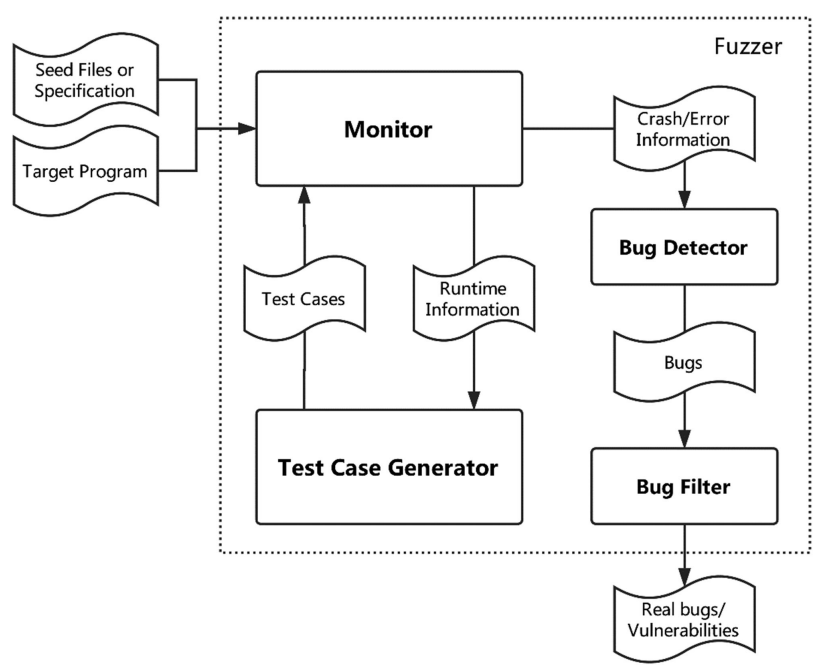
\includegraphics[width = 0.65\textwidth]{../images/Fuzzing.png}
    \caption{Funzionamento generale di un fuzzer. Immagine proveniente da \cite{Fuzzing_soa}}
\end{figure}
Seppur sia una tecnica efficiente e ben conosciuta per effettuare l'analisi di un programma, il fuzzing risente di diverse problematiche, come la necessità, nei fuzzer gray-box e black-box, di generare un input che passi i controlli di sanificazione del programma senza avere
informazioni su quest'ultimo, permettendo così un'analisi più approfondita del programma. Altra problematica è quella legata alla definizione, nei fuzzer mutation-based, di una buona tecnica di mutazione dell'input, in modo da poter analizzare il maggior numero
possibile di cammini di esecuzione interessanti. Per i tool di fuzzing, quindi, la problematica principale da superare è quella di \textbf{implementare una buona strategia di generazione e mutazione dell'input}, in modo tale che essa permetta all'analisi di essere il più approfondita possibile.
\section{Tecniche basate su modelli di apprendimento automatico}
Negli ultimi anni, la ricerca nell'ambito dell'intelligenza artificiale ha compiuto enormi progressi, portando i modelli disponibili ad essere
sempre più accurati ed efficienti. Questo rapido avanzamento ha avuto un impatto significativo anche nel campo della sicurezza informatica, dove
le capacità predittive dell'intelligenza artificiale possono essere sfruttate per l'identificazione automatica di vulnerabilità.
Le tecniche di apprendimento automatico possono essere divise in base a come avviene l'addestramento del modello:
\begin{itemize}
    \item \textbf{Apprendimento supervisionato}: Si sviluppa un modello predittivo tramite l'addestramento su dati etichettati.
    \item \textbf{Apprendimento non supervisionato}: Il modello viene applicato su un insieme di dati non etichettati con lo scopo di trovare una qualche struttura intrinseca del dataset
    \item \textbf{Apprendimento per rinforzo}: Il modello apprende come raggiungere un dato obbiettivo, ricevendo una ricompensa o una penalità in base a quanto la scelta che ha compiuto lo avvicina all'obbiettivo
\end{itemize}
In generale, le tecniche di machine learning per la ricerca di vulnerabilità prevedono l'estrazione di feature significativo dal file binario sotto analisi; le quali verranno poi codificate in un formato idoneo e utilizzate
dal modello per l'identificazione di potenziali percorsi di esecuzione vulnerabili \cite{ML_Survey}.
Sono state proposti diversi approcci basati su machine learning, per esempio \textit{Aumpansub} \& \textit{Huang} \cite{ML1} propongono di estrarre le informazioni sintattiche dal codice assembly e di addestrare
due modelli per il riconoscimento, mentre \textit{Li et al.} \cite{DeepVL} propongono invece di usare come input di addestrare una rete neurale al riconoscimento di vulnerabilità tramite l'utilizzo di tracce di esecuzione del programma ottenute tramite fuzzing.
La ricerca automatica di vulnerabilità in file binari tramite machine learning è un campo relativamente nuovo e, come tale, soffre di alcune problematiche \cite{ML2}:
\begin{itemize}
    \item \textbf{Mancanza della struttura ad alto livello del codice}: Come per l'analisi statica, la mancanza di informazioni sui tipi o sulle funzioni chiamate rende difficile l'applicazione di questo tipo di tecniche
    \item \textbf{Selezione delle feature}: È necessario definire quali sono le feature rilevanti e sviluppare una metodologia per estrarle
    \item \textbf{Selezione del modello}: Bisogna selezionare un modello che permetta di ottenere un grado accettabile di accuratezza. Questo compito è reso particolarmente difficile dal fatto che diversi modelli possono ottenere un'accuratezza comparabile a parità di analisi da effettuare.  
\end{itemize}
\section{Tecniche ibride}
I vari approcci all'analisi di sicurezza presentati fino ad ora non devono essere pensati come insiemi disgiunti. Infatti, la combinazione di queste tecniche è una pratica estremamente diffusa e proficua, visto che permette
di controbilanciare i punti deboli di ciascuna metodologia e di ottenere risultati più accurati. Per esempio, combinare tecniche di analisi statica e dinamica permette di mitigare il numero di falsi positivi ottenuti dalla prima
effettuando un'esplorazione mirata tramite la seconda. Oppure le tecniche di analisi statica e dinamica possono essere usate per ottenere ed estrarre le feature necessarie all'addestramento del modello di riconoscimento (come abbiamo già visto con DeepVL \cite{DeepVL}).




\end{document}